\section{Do we need new imaging phenotypes?}

\newsavebox{\conditions}
\sbox{\conditions}{
    \begin{tikzpicture}
        \begin{groupplot}[
            group style={
                group size=3 by 1,
                horizontal sep=0.2cm
            },
            height=4.5cm,
            width=4.5cm,
            xtick pos=bottom,
            ymajorgrids=true,
            ymajorticks=false,
            ymin=50,
            ymax=100,
            xlabel=\small{Sample size},
            xmin=0,
            tick label style={font=\small},
            title style={font=\small\linespread{0.9}\selectfont\bfseries, anchor=south, yshift=-0.15cm, text depth=0, align=center},
        ]
            \nextgroupplot[
                ymajorticks=true,
                ylabel=Accuracy,
                title=Schizophrenia,
                xtick={0, 500, 1000},
                xticklabels={0, 500, 1000}
            ]
                \addplot[
                    pretrained,
                    only marks,
                    opacity=0.5
                ] table [
                    x=sample,
                    y=accuracy,
                    col sep=comma
                ] {data/SCZ_accuracy_sample.csv};
            \nextgroupplot[
                title={Major Depressive\\Disorder}
            ]
                \addplot[
                    finetune,
                    only marks,
                    opacity=0.5
                ] table [
                    x=sample,
                    y=accuracy,
                    col sep=comma
                ] {data/MDD_accuracy_sample.csv};
            \nextgroupplot[
                title=Bipolar Disorder,
                xtick={0, 1000, 2000, 3000},
                xticklabels={0, 1000, 2000, 3000}
            ]
                \addplot[
                    none,
                    only marks,
                    opacity=0.5
                ] table [
                    x=sample,
                    y=accuracy,
                    col sep=comma
                ] {data/BP_accuracy_sample.csv};
        \end{groupplot}
    \end{tikzpicture}
}

\newsavebox{\counts}
\sbox{\counts}{
    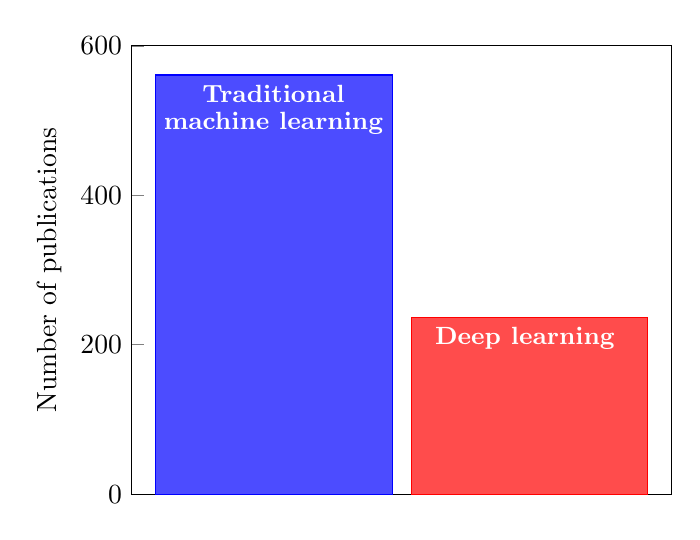
\begin{tikzpicture}
        \begin{axis}[
            ybar,
            ytick pos=left,
            xtick style={draw=none},
            ymin=0,
            ymax=600,
            xmin=-0.5,
            xmax=1.5,
            bar width=3cm,
            xmajorticks=false,
            ylabel=Number of publications
        ]
            \addplot[blue, fill=blue!70] coordinates {
                (0.475, 561)
            };
            \addplot[red, fill=red!70] coordinates {
                (0.525, 236)
            };
            \node[anchor=north, align=center, white, font=\small\linespread{0.9}\selectfont\bfseries] at (axis cs: 0.025, 561) {
                Traditional\\machine learning
            };
            \node[anchor=north, align=center, white, font=\small\linespread{0.9}\selectfont\bfseries] at (axis cs: 0.975, 236) {
                Deep learning
            };
        \end{axis}
    \end{tikzpicture}
}
\newsavebox{\accuracies}
\sbox{\accuracies}{
    \begin{tikzpicture}
        \begin{axis}[
            boxplot/draw direction=y,
            xtick pos=bottom,
            ytick pos=left,
            ylabel=Accuracy,
            xmajorticks=false,
        ]
            \addplot+[
                draw=blue,
                fill=blue!70,
                boxplot prepared={
                    lower whisker=50,
                    lower quartile=74.3,
                    median=82.2,
                    upper quartile=90,
                    upper whisker=100
                },
            ] coordinates {};

            \addplot+[
                draw=red,
                fill=red!70,
                boxplot prepared={
                    lower whisker=72,
                    lower quartile=87.86,
                    median=92,
                    upper quartile=97.13,
                    upper whisker=100
                },
            ] coordinates {};

            \node[anchor=north, align=center, white, font=\footnotesize\linespread{0.85}\selectfont\bfseries] at (axis cs: 1, 90) {
                Traditional\\machine learning
            };
            \node[anchor=north, align=center, white, font=\footnotesize\linespread{0.9}\selectfont\bfseries] at (axis cs: 2, 97.13) {
                Deep learning
            };
        \end{axis}
    \end{tikzpicture}
}

\begin{frame}{Do we need new imaging phenotypes}
    \begin{tikzpicture}
        \node[] at (-5.25, -3.5) {};
        \node[] at (5.25, 3.5) {};

        \visible<1>{
            \node[] (brain) at (-3, 0) {
                \includegraphics[width=2.75cm]{data/mri_sagittal.png}
            };
            \node[] (thinker) at (3, 0) {
                \includegraphics[width=4cm]{data/thinker.png}
            };
            \draw[-stealth, line width=5pt, gray!90] (brain) -- (thinker);
        }
        \visible<2>{
            \node[align=center, anchor=north] at (0, 0.5) {
                \textit{"What I cannot create, I do not understand."}\\
                - Richard Feynman
            };
        }
        \visible<3-4>{
            \node[align=center, anchor=north] at (0, 0.5) {
                \textit{"What I cannot \st{create}, I do not understand."}\\
            };
            \node[] at (-0.5, 0.65) {
                \textit{predict}
            };
        }
        \visible<4>{
            \node[anchor=north, font=\scriptsize] at (0, -0.05) {
                (or I should at least be able to explain why I can't predict it)
            };
        }
        \visible<5>{
            \node[] at (0, 0) {
                \usebox{\conditions}
            };
        }
        \visible<6>{
            \node[] (brain) at (-3, 0) {
                \includegraphics[width=2.75cm]{data/mri_sagittal.png}
            };
            \node[] (thinker) at (3, 0) {
                \includegraphics[width=4cm]{data/thinker.png}
            };
            \draw[-stealth, line width=5pt, gray!90] (brain) -- (thinker);
        }
        \visible<7>{
            \node[] (brain) at (-3, 0) {
                \includegraphics[width=2.75cm]{data/mri_sagittal.png}
            };
            \node[] (thinker) at (3, 0) {
                \includegraphics[width=4cm]{data/thinker.png}
            };
            \draw[-stealth, line width=5pt, red] (brain) -- (thinker);
        }
        \visible<8>{
            \node[] (brain) at (-3, 0) {
                \includegraphics[width=2.75cm]{data/mri_sagittal.png}
            };
            \node[thick, draw=red] (thinker) at (3, 0) {
                \includegraphics[width=4cm]{data/thinker.png}
            };
            \draw[-stealth, line width=5pt, gray!90] (brain) -- (thinker);
        }
        \visible<9>{
            \node[inner sep=0pt, draw=red, very thick] (brain) at (-3, 0) {
                \includegraphics[width=2.75cm]{data/mri_sagittal.png}
            };
            \node[] (thinker) at (3, 0) {
                \includegraphics[width=4cm]{data/thinker.png}
            };
            \draw[-stealth, line width=5pt, gray!90] (brain) -- (thinker);
        }
        \visible<10>{
            \node[] at (0, 0) {
                \usebox{\counts}
            };
        }
        \visible<11>{
            \node[] at (0, 0) {
                \usebox{\accuracies}
            };
        }
    \end{tikzpicture}
\end{frame}
